Our prototype has been written in Java and makes use of the REST API of Kubernetes. 
This component was initially a Java executable that operated outside a Kubernetes cluster,
but at the end it has been shipped inside a container using the building functionality of OpenFaas.
The testing will check two main characteristics: functional requirements and performance.  
\\
\subsubsection*{Functional Requirements}
\paragraph{}
First of all we needed to check if the Kubernetes API was reachable from our code.
The first executable was configured to access a cluster from outside. This was done by loading
the administrator configuration file in the API.
The limit of this method was that the component had to be launched on the administrator machine with a JVM
and that it had full control of the cluster. 
\\
These problems were solved by building a container with our executable by using OpenFaas and deploying it
in the cluster.
\\
In Kubernetes permissions are granted to pods by creating new Roles. These are objects that tell which API 
calls can be made by an agent inside the cluster, and can specify which objects can be affected by these calls.
\\
Since a running pod does not have access to the old configuration file (because it's not deployed on the administrator machine),
it didn't have the permission to read and updated nodes' labels, and so we had to link it to a Role.
After doing this procedure, the behavior of the component inside and outside the cluster is identical,
since it does not affect the SLPA code.
\paragraph{}
For what concerns SLPA, the algorithm in the container runs only if the nodes that
are given as input are registered inside the Kubernetes cluster. Since this check does not have
any effect on the execution of the algorithm and requires the presence of real hosts in a network,
we decided to unit-test the algorithm locally outside the container.
We created a dummy network \ref{fig:RR2} by filling the delay matrix and giving it to the algorithm.
The delay matrix is a  $NxN$ matrix, where N is the number of nodes of the network.
The cell M[$i$,$j$] contains the delay between the node $i$ and $j$. If this
cell is set to -1, there is no arc that links the two nodes. A delay threshold given as input will set to -1
all the cells that have a delay greater than that. In this example, the network shown is the one obtained after 
deleting all of these arcs that have a too high delay. The delays are not shown in the figure in order
to keep the visualization simple and because SLPA does not consider the value of the arcs but only their presence.
Note that in a real world scenario this delay would be measured for example by pinging the target node.
\par
Figure \ref{fig:netNoRR} shows the result of the algorithm without Round Robin. In this output the size of the 
different communities varies a lot. Since SLPA makes some decision based on chance, reapplying the
algorithm on the same network will give different results, creating each time different communities.
Figure \ref{fig:RR1} and \ref{fig:RR2} shows the effects of the Round Robin on the communities that were exceeding 
in size. In this examples, the maximum size of a community was set to 5. In figure \ref{fig:RR1} SLPA returned
two communities, one that included all the nodes from 1 to 8 while the other one included the remaining ones.
These were broken down  by the RR, creating 4 communities that cannot be broken down in 4 different partitions.
Figure \ref{fig:RR2} shows a luckier iteration of SLPA, that returned only one oversized community (from node 9
to node 15). 
\\
The fact that some nodes are not directly connected to the others of the same community is not a problem,
since sometimes also SLPA outputs communities with a structure similar to the one returned by the Round Robin in these examples.
However, if SLPA returns a very large community, with size larger than the maximum size allowed, a set of communities
with disconnected nodes could be created, since there is no logic that tries to group closer nodes.
This result would be not optimal, since for sure exists another configuration that can have lower
overall delay between the nodes of a community.


\begin{figure}[]
    \centering
    \subfloat[Dummy Netowrk]{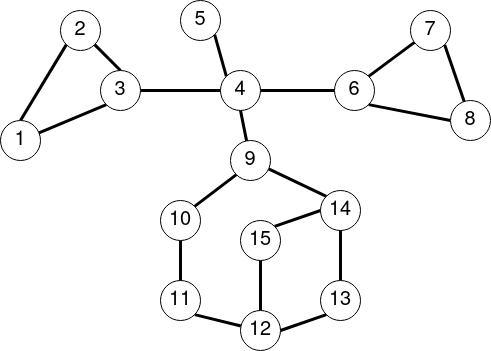
\includegraphics[width=.45\linewidth]{Images/rete.png}
    \label{fig:network}}
    \subfloat[SLPA without RR]{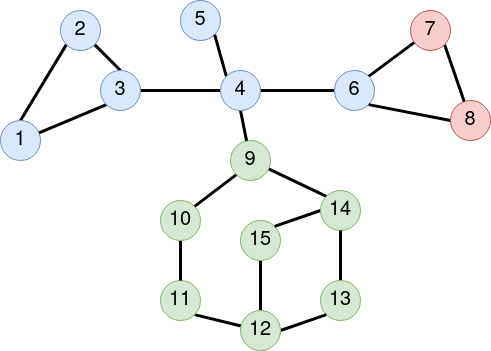
\includegraphics[width=.45\linewidth]{SLPAnoLimit.png}
    \label{fig:netNoRR}}
    \\
    \subfloat[SLPA with RR]{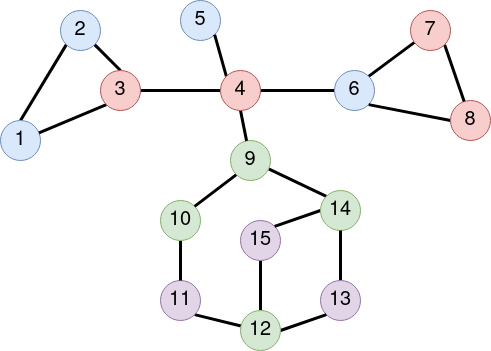
\includegraphics[width=.45\linewidth]{SLPARR5.png}
    \label{fig:RR1}}
    \subfloat[SLPA with RR]{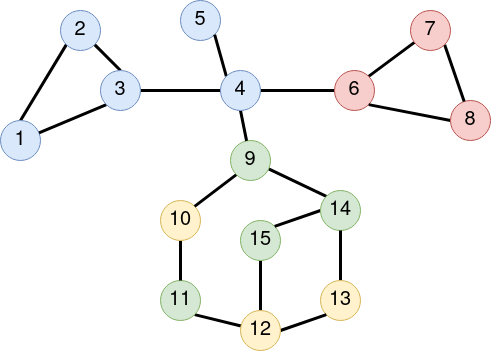
\includegraphics[width=.45\linewidth]{SLPARR5good.png}
    \label{fig:RR2}}
\end{figure}






\subsubsection*{Perfomance}




\begin{figure}[]
    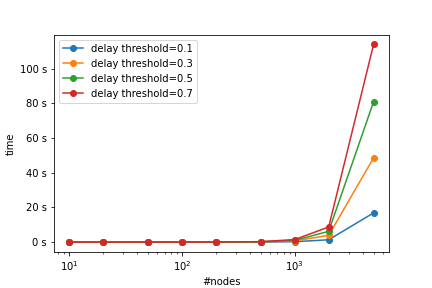
\includegraphics[width=\textwidth]{node.png}
    \label{fig:plotCommunity}
    \caption{PAPS general structure}
\end{figure}

\begin{figure}[]
    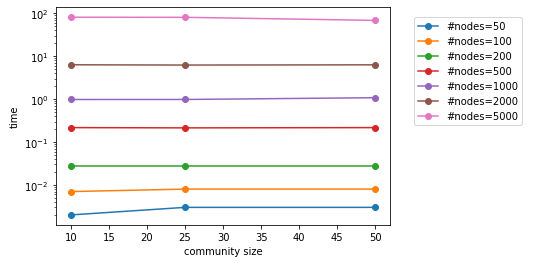
\includegraphics[width=\textwidth]{communitySize.png}
    \label{fig:plotSize}
    \caption{PAPS general structure}
\end{figure}



Parte di testing divisa in funzionale e non funzionale

FUNZIONALE
1) testing dell'integrazione con kubernetes.
    si può fare dentro o fuori, cambiano i permessi.
    una volta settati, 'algoritmo può essere chiamato in remoto senza alcun cambiamento nel comportamento
    Unit test sulle singole chiamate dentro e fuori il cluster?

2) testing sulle reti prodotte da SLPA con esempi (disegnati con draw-io)
    delay matrix: se un link tra il nodo i e j esiste, la cella i j+ un numero positivo che contiene il delay tra i
    due. Se un link non è presente, la cella è settata a -1 
    direi quella da 10 nodi che abbiamo fatto. Poi facciamo la stessa rete ma con una size delle 
    community più piccola per vedere come triggera il round robin (magari in diverse iterazioni)

NON FUNZIONALE:
1) testare l'algoritmo su openFaas non ha senso, è in localhost e non da nessun insight

2) testing del nostro SLPA con una rete generata casualmente, tagliamo i nodi e vediamo  con diverse size
    e con diverse delay threshold come cambiano le performance
    considerazioni su presenza di round robin e altro.










Since our code has been shipped inside a container, we needed to test if the prototype
was able to communicate with the chosen frameworks. In fact, the partition module  needs to invoke the Kubernetes API
in order to assign the community and role labels.\\
We deployed our container on Minikube. Minikube is a virtual machine running in VirtualBox, in which a
one-node Kubernetes cluester has already been deployed. The deployment of the container 
was done by using the OpenFaas CLI, and its functionalities were tested by using both the invocation
through the \textit{faas-cli} and the \textit{faas-gui}.\\
The SLPA algorithm was tested locally by creating a mock delay matrix. This matrix should be symmetric and, 
in order to have significant results, it should reflect the structure of a real network. In fact, drawing the network
delays from a uniform distribution produces a single community in which all nodes have been put but doesn't correspond
to any real-world network.
When applied to a correctly build matrix, the algorithm works as expected. The big communities broken down by our Round Robin 
implementation are still correct, but they look more sparse, since the assignment to the new smaller communities is done by
cycling on an unordered list.